\documentclass[border=6pt]{standalone}
\usepackage{amsmath,amssymb}
\usepackage{tikz}
\usepackage{pgfplots}
\pgfplotsset{compat=1.18}

\begin{document}

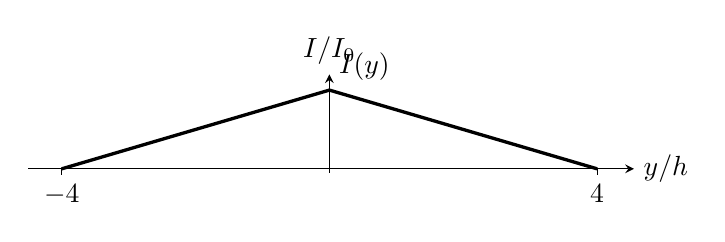
\begin{tikzpicture}[x=0.85cm,y=1.0cm,>=stealth]
  \draw[->] (-4.5,0)--(4.55,0) node[right] {$y/h$};
  \draw[->] (0,-0.05)--(0,1.2) node[above] {$I/I_0$};
  \draw[very thick] (-4,0)--(0,1)--(4,0);
  \draw[dashed] (-4,0)--(-4,-0.08) node[below] {$-4$};
  \draw[dashed] (4,0)--(4,-0.08) node[below] {$4$};
  \node[above right] at (0,1) {$I(y)$};
\end{tikzpicture}

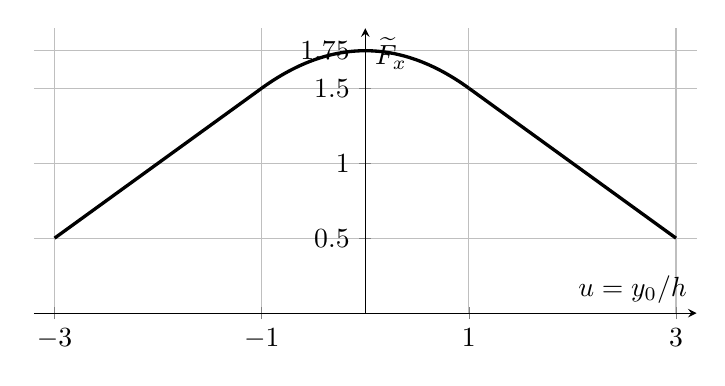
\begin{tikzpicture}
  \begin{axis}[
    width=10cm,height=5.2cm,
    axis lines=middle,
    xmin=-3.2,xmax=3.2,ymin=0,ymax=1.9,
    xlabel={$u=y_0/h$},
    ylabel={$\widetilde F_x$},
    xtick={-3,-1,0,1,3},
    ytick={0,0.5,1,1.5,1.75},
    grid=both,
    samples=2
  ]
    \addplot[very thick,domain=-3:-1] {(4+x)/2};
    \addplot[very thick,domain=-1:1,samples=100] {(7-x^2)/4};
    \addplot[very thick,domain=1:3] {(4-x)/2};
  \end{axis}
\end{tikzpicture}

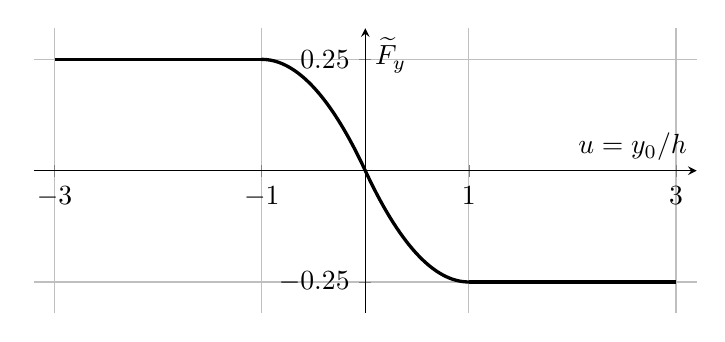
\begin{tikzpicture}
  \begin{axis}[
    width=10cm,height=5.2cm,
    axis lines=middle,
    xmin=-3.2,xmax=3.2,ymin=-0.32,ymax=0.32,
    xlabel={$u=y_0/h$},
    ylabel={$\widetilde F_y$},
    xtick={-3,-1,0,1,3},
    ytick={-0.25,0,0.25},
    grid=both,
    samples=2
  ]
    \addplot[very thick,domain=-3:-1] {1/4};
    \addplot[very thick,domain=-1:0,samples=100] {-x*(x+2)/4};
    \addplot[very thick,domain=0:1,samples=100] {x*(x-2)/4};
    \addplot[very thick,domain=1:3] {-1/4};
  \end{axis}
\end{tikzpicture}

\end{document}
